% Extensionly - análise e projeto de software, artefatos da implementação, maior capítulo de todos, modelo de domínio, diagrama de componentes, paradigma de programação, tecnologias, processo da engenharia de software, separação frontend/backend (com mais detalhes técnicos), usar figuras e modelos
% seção devops
% seção analytics
%=======================================
\chapter{Extensionly Front-end Design}\label{extensionly}
%=======================================

This chapter describes how the solution will be developed and the process behind its implementation, presenting information about the applied software engineering to create the system. In \Cref{ext:initial-considerations}, it is briefly presented how the front-end relates to the other \ac{TP} written about Extensionly, which focuses on the back-end implementation. The chapter also discusses user roles. \Cref{ext:requirement-engineering} presents how the system requirements were managed. Lastly, \Cref{ext:design-decisions} presents some of the design decisions made in order to develop a robust application.

It is also important to note that the terms ``front-end'', ``system'', ``application'', ``web app'' and ``tool'' are used interchangeably to refer to the goal product of this study.

\section{Initial Considerations}\label{ext:initial-considerations}

The Extensionly front-end will be developed as a web application, which relates to the back-end by consuming its \ac{API}, - a collection of established guidelines that describe how programs or computers communicate with one another \cite{ibmapi}. The project will be versioned using Git, a version control system made to manage any project, no matter how big or small, quickly and effectively \cite{chacon2014pro}. The source code will be available in the official repository\footnote{Extensionly front-end code is available at \url{https://github.com/Dalepfell/extensionly-frontend}}. A lot of communication between both authors is required for the partnership to work, since this is the only client being developed for the back-end server for now.

In addition to assisting various university outreach activities, the tool's overall goal is to improve ties between the academic and outside communities by opening a line of contact through which requests can be made to the university.
As a result, students will get more familiar with and connected to the community as a whole, which will greatly benefit their formation.

The tool's primary application is for \ac{UNIPAMPA} Campus Alegrete, but it may also be utilized by other campuses within the university system and potentially by other Brazilian institutions in the future.

\section{Requirements Engineering}\label{ext:requirement-engineering}

This sections aims to present in more detail how the requirements were collected and refined throughout the study. There were two (2) steps to the requirements elicitation stage. The first batch is the result of the grey literature systematic review described in detail in \Cref{greyliterature}. The second refinement of the requirements was applied after analyzing the survey results, presented earlier in \Cref{survey}.

\subsection{Requirements Obtained through the Grey Literature Review}\label{ext:requirements-grey}

In total, twenty eight (28) \acp{FR} were defined prior to the planning and execution of the survey. \textcite{Clarkson2005-sy} explain that \acp{FR} have the purpose to establish the behavior between inputs and outputs that characterizes a system's or component's function.

These requirements were created after analyzing other tools found during the grey literature review, presented earlier in \Cref{sec:gl-feature-matrix}, which had similar scope to the system being developed. Out of these requirements, six (6) of them were ruled out for now after discussions between both authors and their supervisor, due to some of them being too complex for an \ac{MVP} or simply out of scope. The remaining twenty two (22) were prioritized based on what was considered most critical for the application \ac{MVP}. The complete list of initial requirements and their priority ranking can be seen in \Cref{tab:initial-requirements}.

\begin{table}[!htb]
  \centering
  \setlength{\aboverulesep}{0pt}
  \setlength{\belowrulesep}{0pt}
  \caption{Initial Requirements}
  \label{tab:initial-requirements}
  \footnotesize
  \begin{tabular}{c|l|c}
    \toprule
    \rowcolor[rgb]{0.753,0.753,0.753} \textbf{ID} & \multicolumn{1}{c|}{\textbf{Requirement}}                    & \textbf{Priority} \\
    \hline
    \rowcolor[rgb]{0.898,0.898,0.898} FR. 01      & Propose new OAs                                              & High              \\
    FR. 02                                        & Allow enrollments in OA                                      & High              \\
    \rowcolor[rgb]{0.898,0.898,0.898} FR. 03      & Record participant attendance                                & High              \\
    FR. 04                                        & Review and approve OA proposals                              & High              \\
    \rowcolor[rgb]{0.898,0.898,0.898} FR. 05      & Text search for OAs                                          & High              \\
    FR. 06                                        & Registration of OA prerequisites                             & High              \\
    \rowcolor[rgb]{0.898,0.898,0.898} FR. 07      & Edit enrollment status in OAs                                & High              \\
    FR. 08                                        & List OAs the user is enrolled in                             & High              \\
    \rowcolor[rgb]{0.898,0.898,0.898} FR. 09      & Maintain history of OAs participated                         & High              \\
    FR. 10                                        & Help area (frequently asked questions, manuals)              & High              \\
    \rowcolor[rgb]{0.898,0.898,0.898} FR. 11      & OAs query with filter                                        & Medium            \\
    FR. 12                                        & External user registration                                   & Medium            \\
    \rowcolor[rgb]{0.898,0.898,0.898} FR. 13      & Registration of interest in areas of knowledge               & Medium            \\
    FR. 14                                        & Show proponent details                                       & Medium            \\
    \rowcolor[rgb]{0.898,0.898,0.898} FR. 15      & Favorites list for OAs                                       & Medium            \\
    FR. 16                                        & Declare interest in an OA (when enrollments are not open)    & Medium            \\
    \rowcolor[rgb]{0.898,0.898,0.898} FR. 17      & Share OA information                                         & Medium            \\
    FR. 18                                        & OA past versions history                                     & Medium            \\
    \rowcolor[rgb]{0.898,0.898,0.898} FR. 19      & Teacher's note in the OA details                             & Medium            \\
    FR. 20                                        & Final OA assessment by the student                           & Medium            \\
    \rowcolor[rgb]{0.898,0.898,0.898} FR. 21      & Detailed schedule for upcoming OAs                           & Low               \\
    FR. 22                                        & Fill in final OA report~                                     & Low               \\
    \rowcolor[rgb]{0.898,0.898,0.898} FR. 23      & Print enrollment status                                      & Removed           \\
    FR. 24                                        & Testimonies/reviews from past participants in the OA details & Removed           \\
    \rowcolor[rgb]{0.898,0.898,0.898} FR. 25      & Instructor/student communication channel                     & Removed           \\
    FR. 26                                        & Environment for evaluation of students submitted works       & Removed           \\
    \rowcolor[rgb]{0.898,0.898,0.898} FR. 27      & List of OAs by teacher                                       & Removed           \\
    FR. 28                                        & List of related OAs                                          & Removed           \\
    \bottomrule
  \end{tabular}
\end{table}

The following are sketches of how the initial requirements relate to the defined user roles. \Cref{fig:use-case-1} presents the first 14 \ac{FR} and \Cref{fig:use-case-2}, the remaining 8, excluding the ones that were removed.

\begin{figure}[!htb]
  \caption{User Roles on the First 14 \ac{FR}}\label{fig:use-case-1}
  \begin{center}
    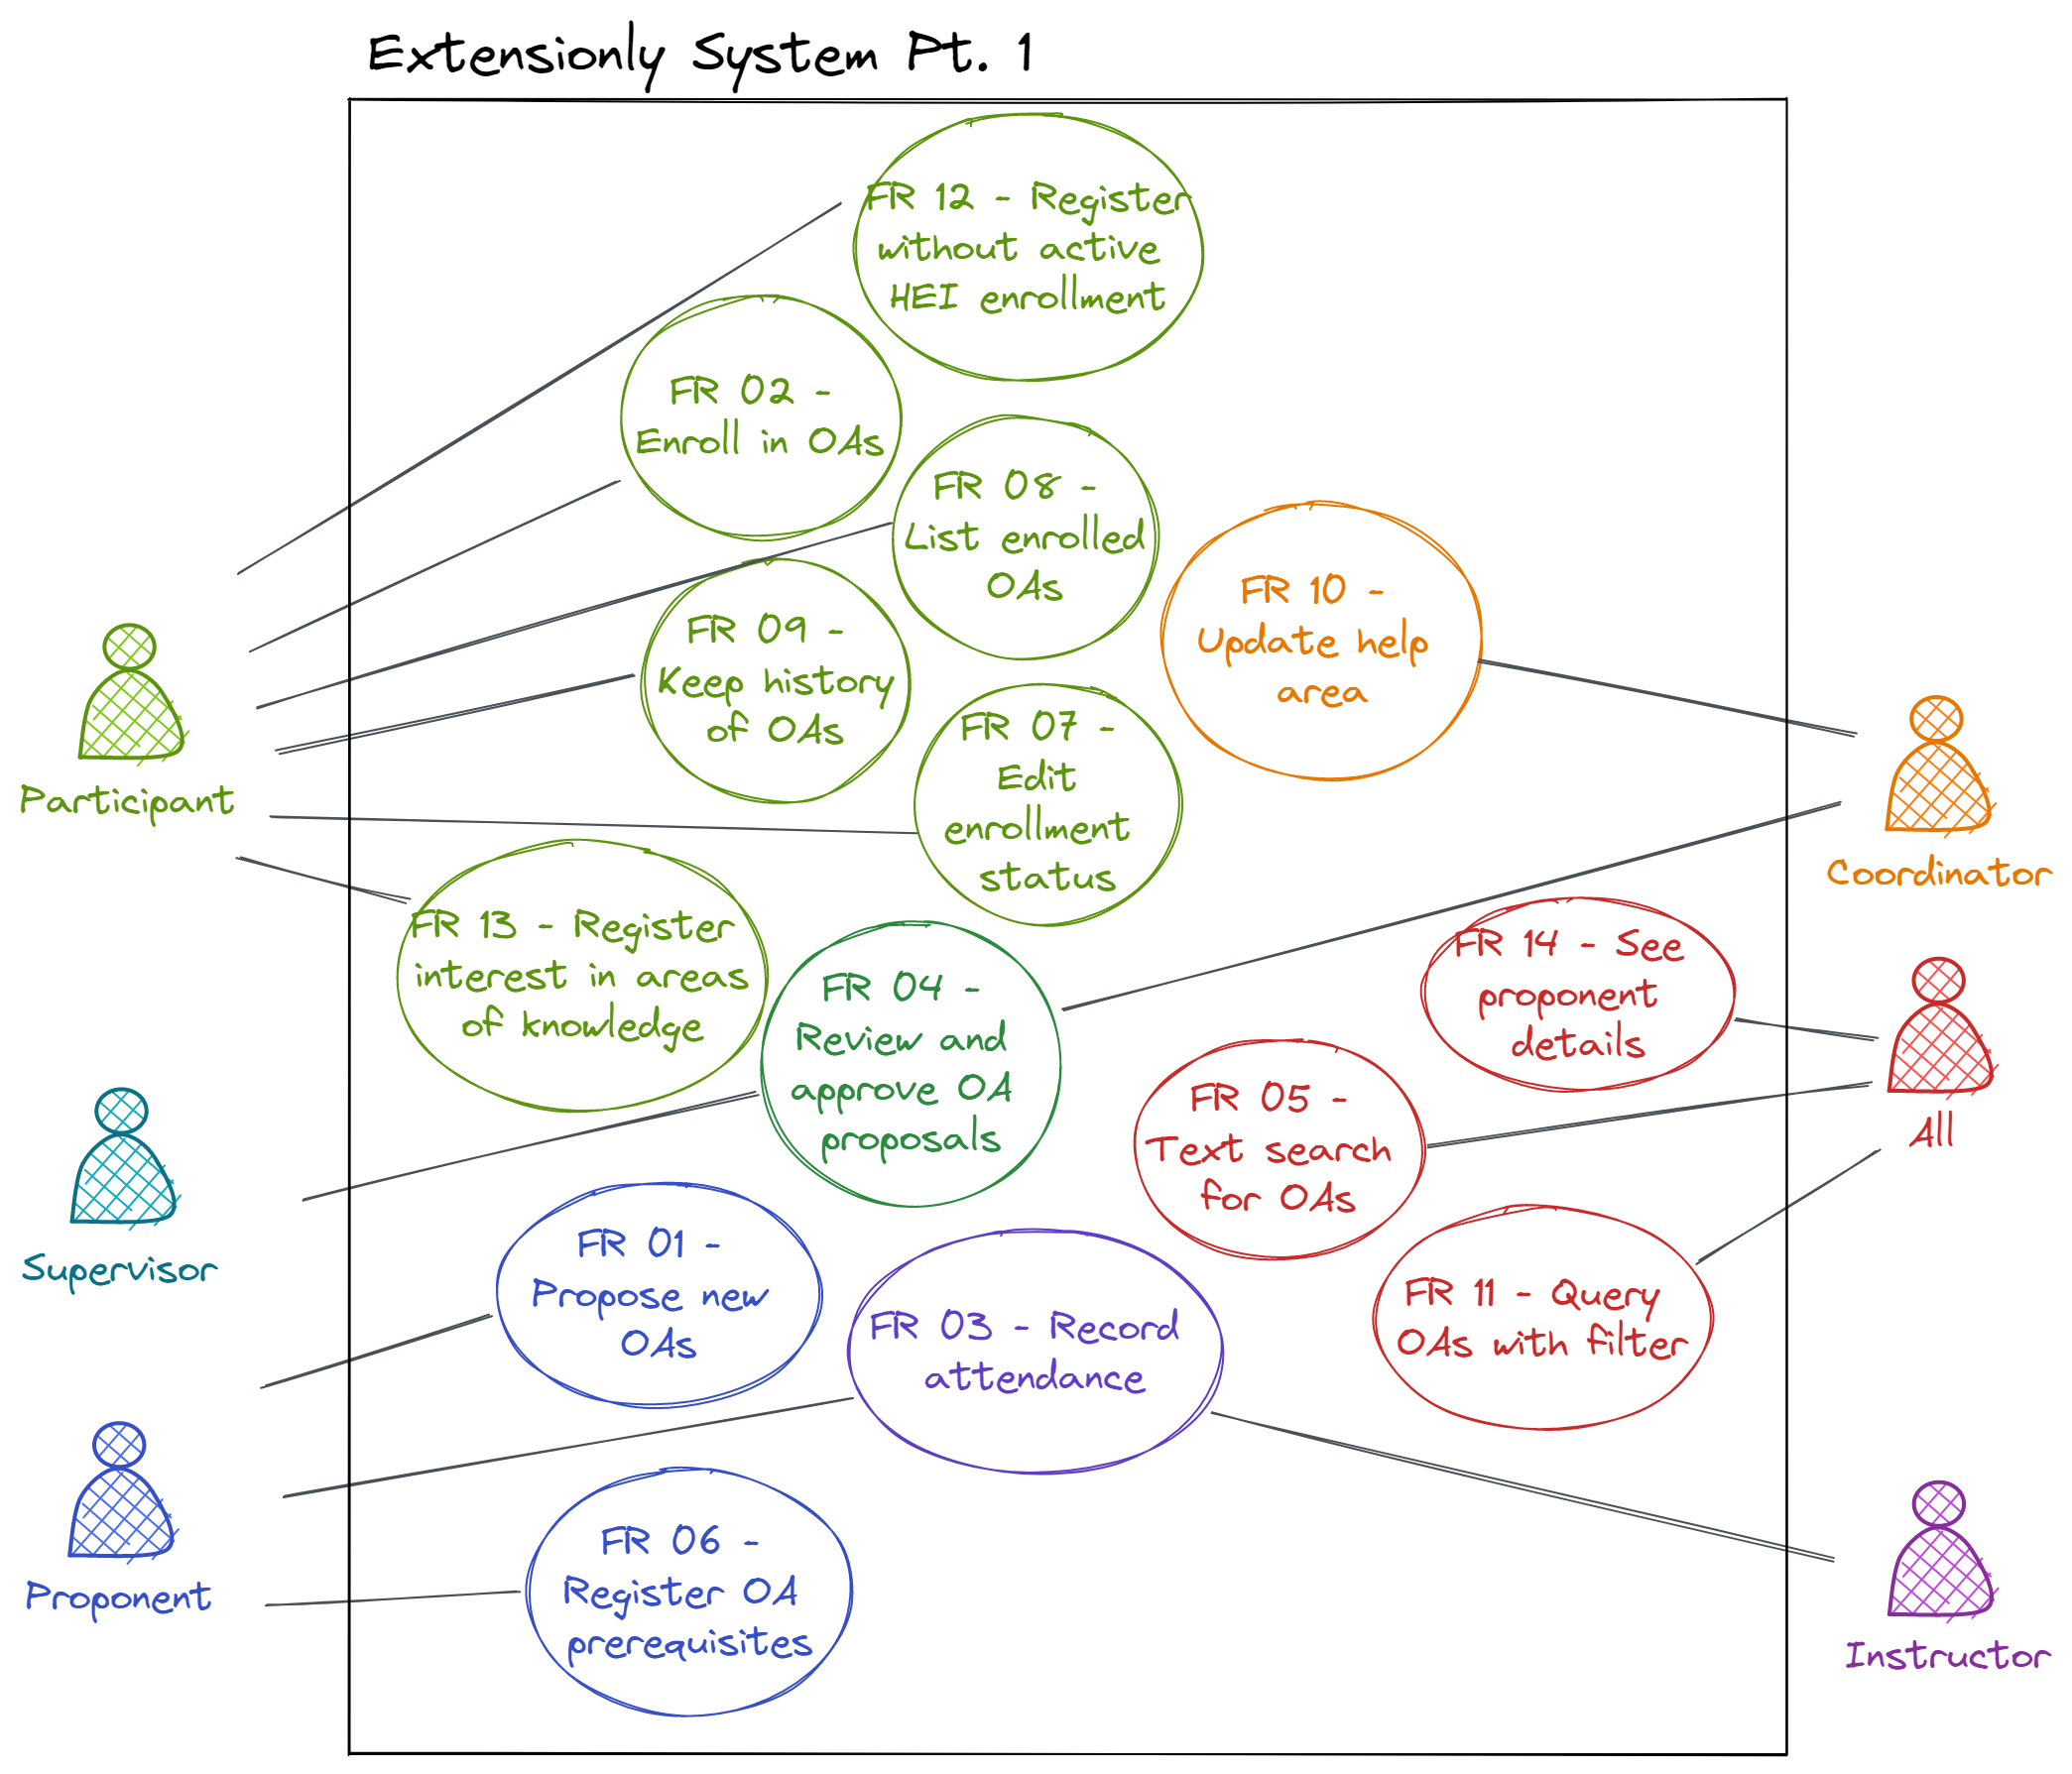
\includegraphics[width=15cm]{img/6-use-case-1.png}
  \end{center}
  \fonte{Author.}
\end{figure}

\begin{figure}[!htb]
  \caption{User Roles on the Last 8 \ac{FR}}\label{fig:use-case-2}
  \begin{center}
    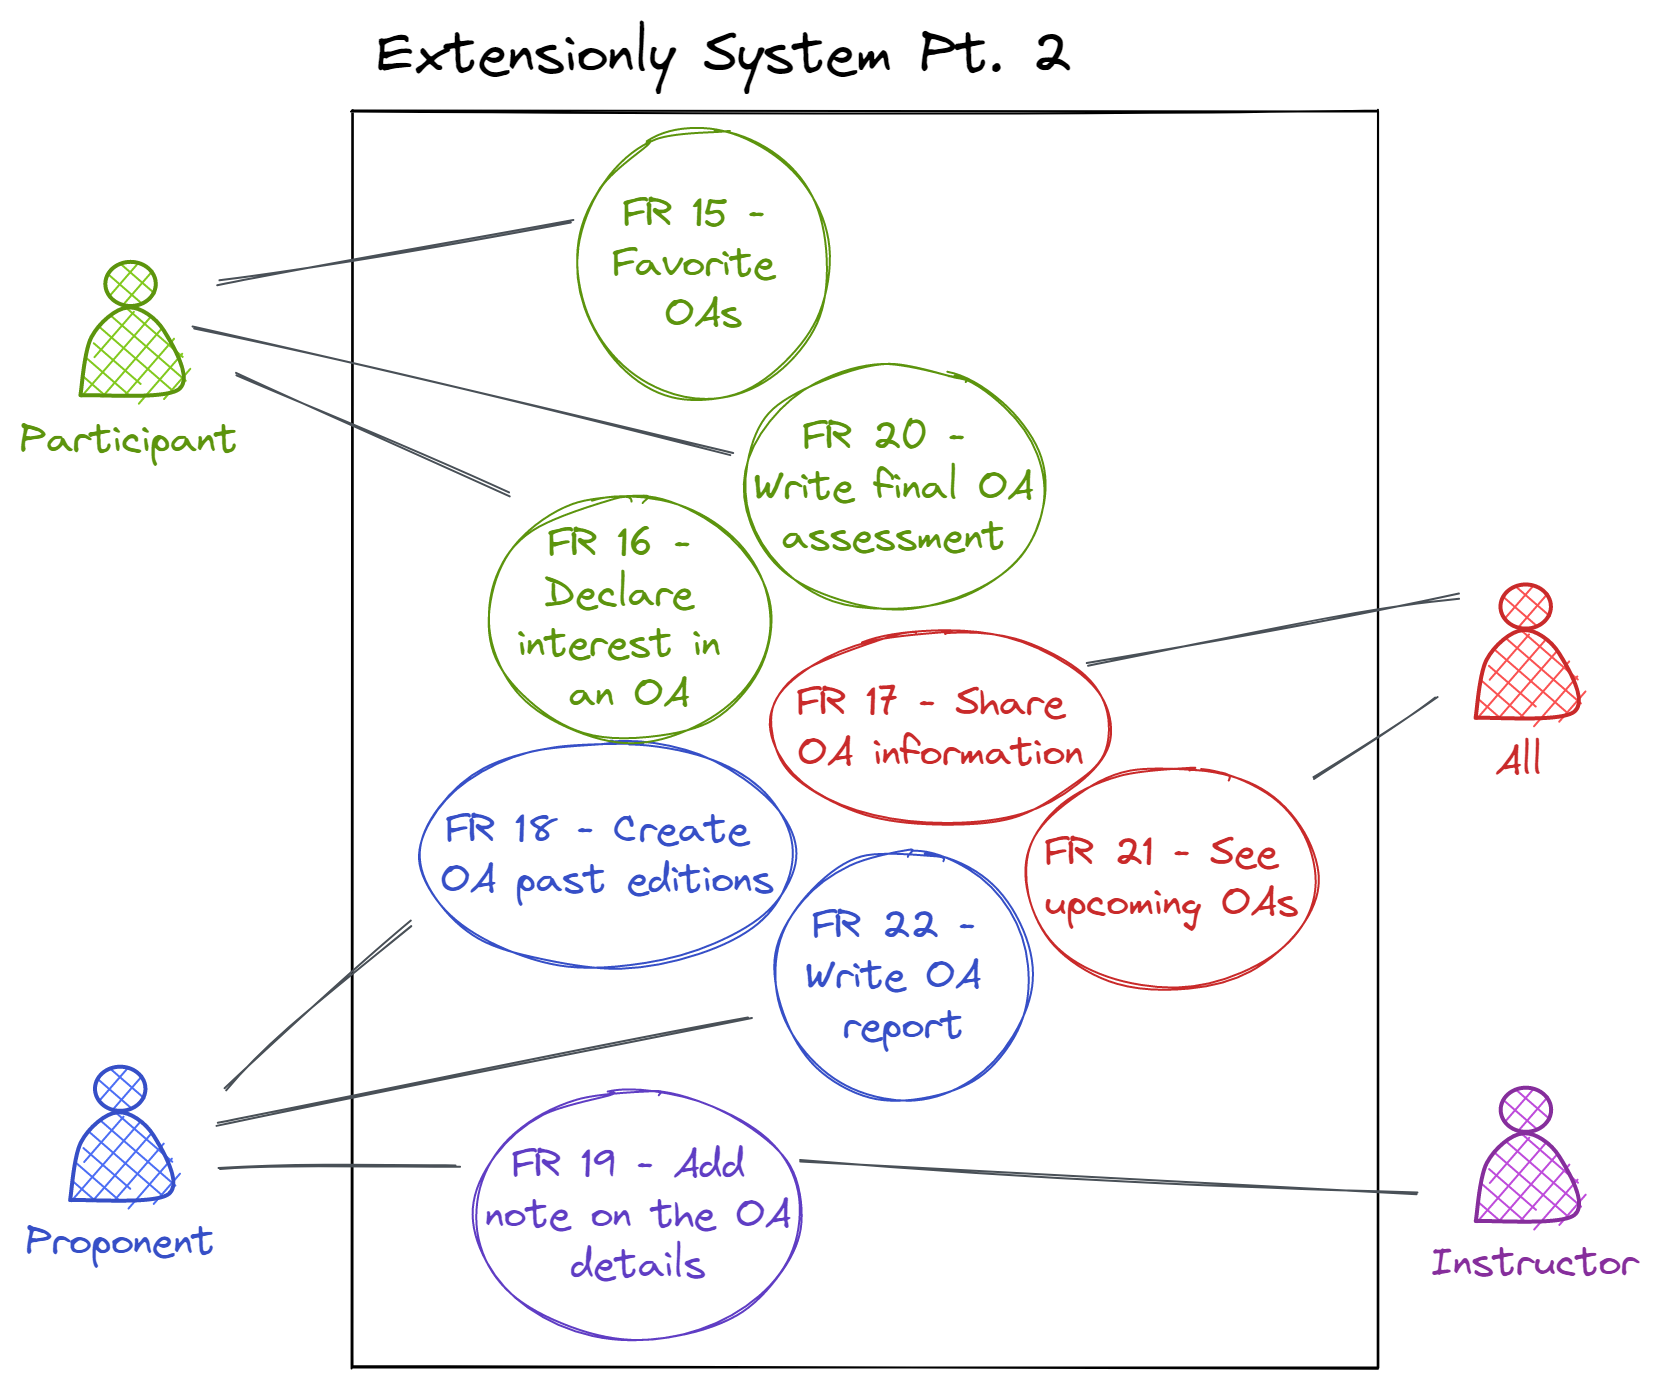
\includegraphics[width=12cm]{img/6-use-case-2.png}
  \end{center}
  \fonte{Author.}
\end{figure}

\subsection{User Stories derived from the Requirements}\label{ext:user-stories}

After the first round of defining the \acp{FR}, it was necessary to turn them into user stories, to use them in the survey, in a more descriptive form for the respondents. The stories were written with the system user roles in mind, which were presented earlier in \Cref{ext:initial-considerations}. They were used directly, with no other refinements, in the final survey and were defined in \Cref{tab:proponent-user-stories}, \Cref{tab:instructor-user-stories}, \Cref{tab:participant-user-stories} and \Cref{tab:coordinator-user-stories}.

\begin{table}[!htb]
  \centering
  \setlength{\aboverulesep}{0pt}
  \setlength{\belowrulesep}{0pt}
  \caption{Proponent User Stories}
  \label{tab:proponent-user-stories}
  \footnotesize
  \begin{tabularx}{\textwidth}{c|X}
    \toprule
    \rowcolor[rgb]{0.753,0.753,0.753} \textbf{ID} & \textbf{User Story}                    \\
    \hline
    \rowcolor[rgb]{0.898,0.898,0.898} P1          & As a Proponent, I would like to propose an outreach activity, creating knowledge opportunities for other people.                                           \\
    P2                                            & As a Proponent, I would like to define desired prerequisites for enrollment in my outreach activity proposal, so that my applicants do not come unprepared.                                      \\
    \rowcolor[rgb]{0.898,0.898,0.898} P3          & As a Proponent, I would like my data to be shown along the details page of my outreach activity, so that participants have more details of who I am.                                \\
    P4                                            & As a Proponent, I would like to leave comments on the outreach activity page, to request some special material for carrying out the activity or just leave a note of mine for the participants.                              \\
    \rowcolor[rgb]{0.898,0.898,0.898} P5          & As a Proponent, I would like to fill in a general report on the progress of the outreach activity carried out, for archiving purposes.                                \\
    P6                                            & As a Proponent, I would like to register multiple editions of the same outreach activity, so that new participants can check past editions.                              \\
    \rowcolor[rgb]{0.898,0.898,0.898} P7          & As a Proponent or Instructor, I would like to get in touch with the participants of the outreach activity, so that it is easy to pass on information relevant to the activity.                                \\
    P8                                            & As a Proponent, I would like to receive the evaluation of the participants of my outreach activity in a detailed report/form format, so that I am aware of what I should improve for the next edition.                              \\
    \bottomrule
  \end{tabularx}
\end{table}
\begin{table}[!htb]
  \centering
  \setlength{\aboverulesep}{0pt}
  \setlength{\belowrulesep}{0pt}
  \caption{Instructor User Stories}
  \label{tab:instructor-user-stories}
  \footnotesize
  \begin{tabularx}{\textwidth}{c|X}
    \toprule
    \rowcolor[rgb]{0.753,0.753,0.753} \textbf{ID} & \multicolumn{1}{c}{\textbf{User Story}}                    \\
    \hline
    \rowcolor[rgb]{0.898,0.898,0.898} I1          & As an Instructor, I would like to manage the attendance of registered participants so that certificates can be issued for those present.                                           \\
    \bottomrule
  \end{tabularx}
\end{table}
\begin{table}[!htb]
  \centering
  \setlength{\aboverulesep}{0pt}
  \setlength{\belowrulesep}{0pt}
  \caption{Participant User Stories}
  \label{tab:participant-user-stories}
  \footnotesize
  \begin{tabularx}{\textwidth}{c|X}
    \toprule
    \rowcolor[rgb]{0.753,0.753,0.753} \textbf{ID} & \multicolumn{1}{c}{\textbf{User Story}}                    \\
    \hline
    \rowcolor[rgb]{0.898,0.898,0.898} A1          & As a Participant, I would like to apply for outreach activities such as events, courses and lectures, to enter the waiting list and be accepted in the activity.                                          \\
    A2                                            & As a Participant, I would like to be able to search for outreach activities, so that I can find what I am looking for more easily.                                     \\
    \rowcolor[rgb]{0.898,0.898,0.898} A3          & As a Participant, I would like to cancel or edit the information of an outreach activity enrollment made by me, to have more freedom in case I change my mind.                                \\
    A4                                            & As a Participant, I would like to see previous editions of outreach activities, so that I can read past proposals.                              \\
    \rowcolor[rgb]{0.898,0.898,0.898} A5          & As a Participant, I would like to view the history of all the outreach activities I have participated in, so that I don't have to keep the record outside of the tool.                                \\
    A6                                            & As a Participant, I would like to have a help area within the system, to guide me with any questions or problems that I may face with the activity I signed up for.                              \\
    \rowcolor[rgb]{0.898,0.898,0.898} A7          & As a Participant without college enrollment, I would like to register in the system to participate in outreach activities that interest me.                                \\
    A8                                            & As a Participant, I would like to inform my interest in areas of knowledge, so that I can see outreach activities related to them.                              \\
    \rowcolor[rgb]{0.898,0.898,0.898} A9          & As a Participant, I would like to favor outreach activities that I deem interesting, so that I have easy access to them when I need them.                                \\
    A10                                           & As a Participant, I would like to show my interest in unavailable outreach activities, so that I will be notified when a new issue opens.                              \\
    \rowcolor[rgb]{0.898,0.898,0.898} A11         & As a Participant, I would like to register for outreach activities without registering in the system, so that my information is not saved.                                \\
    A12                                           & As a Participant, I would like to share information about the outreach activity, so that I can share it more easily with my friends.                              \\
    \rowcolor[rgb]{0.898,0.898,0.898} A13         & As a Participant, I would like to evaluate the outreach activity in which I participated, so that other participants can see the grade I assigned.                                \\
    A14                                           & As a Participant, I would like to see the outreach activities in which I am enrolled in the form of a calendar, so that I can organize myself better.                              \\
    \bottomrule
  \end{tabularx}
\end{table}
\begin{table}[!htb]
  \centering
  \setlength{\aboverulesep}{0pt}
  \setlength{\belowrulesep}{0pt}
  \caption{Coordinator User Stories}
  \label{tab:coordinator-user-stories}
  \footnotesize
  \begin{tabularx}{\textwidth}{c|X}
    \toprule
    \rowcolor[rgb]{0.753,0.753,0.753} \textbf{ID} & \multicolumn{1}{c}{\textbf{User Story}}                    \\
    \hline
    \rowcolor[rgb]{0.898,0.898,0.898} C1          & As Coordinator, I would like to manage the submissions of new outreach activities carried out, so that each proposal goes through a review process before being accepted.                                           \\
    C2                                            & As Coordinator, I would like to issue certificates of participation with a certain number of hours for all involved, participants, instructors and coordinator, so that the individual's involvement in the outreach activity is proven.                                     \\
    \bottomrule
  \end{tabularx}
\end{table}

However, in order to relate \acp{FR} with the questions and also update their ranking based on the survey results, \Cref{tab:stories-requirements-relation} was created.

\begin{table}[!htb]
  \centering
  \setlength{\aboverulesep}{0pt}
  \setlength{\belowrulesep}{0pt}
  \caption{User Stories}
  \label{tab:stories-requirements-relation}
  \footnotesize
  \begin{tabular}{c|c|c}
    \toprule
    \rowcolor[rgb]{0.753,0.753,0.753} \textbf{Requirement ID} & \textbf{Question/story ID} & \textbf{Priority} \\
    \hline
    \rowcolor[rgb]{0.898,0.898,0.898} FR. 01                  & P1                         & Must have         \\
    FR. 02                                                    & A1                         & Must have         \\
    \rowcolor[rgb]{0.898,0.898,0.898} FR. 03                  & I1                         & Must have         \\
    FR. 04                                                    & C1                         & Must have         \\
    \rowcolor[rgb]{0.898,0.898,0.898} FR. 05                  & A2                         & Must have         \\
    FR. 06                                                    & P2                         & Should have       \\
    \rowcolor[rgb]{0.898,0.898,0.898} FR. 07                  & A3                         & Must have         \\
    FR. 08                                                    & A5                         & Must have         \\
    \rowcolor[rgb]{0.898,0.898,0.898} FR. 09                  & A5                         & Must have         \\
    FR. 10                                                    & A6                         & Must have         \\
    \rowcolor[rgb]{0.898,0.898,0.898} FR. 11                  & A2                         & Must have         \\
    FR. 12                                                    & A11                        & Will not have     \\
    \rowcolor[rgb]{0.898,0.898,0.898} FR. 13                  & A8                         & Must have         \\
    FR. 14                                                    & P3                         & Should have       \\
    \rowcolor[rgb]{0.898,0.898,0.898} FR. 15                  & A9                         & Must have         \\
    FR. 16                                                    & A10                        & Must have         \\
    \rowcolor[rgb]{0.898,0.898,0.898} FR. 17                  & A12                        & Should have       \\
    FR. 18                                                    & P6                         & Must have         \\
    \rowcolor[rgb]{0.898,0.898,0.898} FR. 19                  & P4                         & Should have       \\
    FR. 20                                                    & A13                        & Should have       \\
    \rowcolor[rgb]{0.898,0.898,0.898} FR. 21                  & A14                        & Must have         \\
    FR. 22                                                    & P5                         & Should have       \\
    \bottomrule
  \end{tabular}
\end{table}

There were some cases where multiple \acp{FR} were assigned to a single user story, because the requirements are usually more technical, while a user story is supposed to have a higher level of abstraction \cite{DIMITRIJEVIC2015352}.

\subsubsection{User Roles}\label{ext:user-roles}

The system as a whole, including the back-end service, was designed with multiple user roles, or actors, in mind. According to \textcite{omg_2017}, in the Unified Modeling Language, an actor designates a function performed by a user or by any other system that communicates with the subject. In this case, it was referred as the user.

This was a necessity identified very early on, since there are many actors involved in the \ac{OA} ecosystem in \acp{HEI}, as was presented earlier in the study. They are as follows:
\begin{description}
  \item[\textbf{Participant}] - a listener, someone who enrolls to passively participate in the activity;
  \item[\textbf{Instructor}] - a speaker, someone who presents or teaches something to participants;
  \item[\textbf{Proponent}] - the one who proposes the \ac{OA}, usually a professor;
  \item[\textbf{Coordinator}] - a role that can review and approve proposed activities for one campus;
  \item[\textbf{Supervisor}] - usually does not interact with the process, but can monitor the system as a whole, having access to \ac{OA} in multiple campuses.
\end{description}
Initially, there was also an ``External Participant'' role, whose difference from the Participant was that no \ac{HEI} enrollment was required in order for it to enroll in \acp{OA}. It is being put on hold for now, because it is considered to be somewhat out of scope of an \ac{MVP}.

\section{Design Decisions}\label{ext:design-decisions}

The decisions made regarding the development of the goal product are discussed in this section.

\begin{description}
  \item[\textbf{Programming Language:}] \ac{TS} was chosen because of the incredible ecosystem of tools and technologies built around it. It expands the capabilities of common \ac{JS}, a dynamic typed language, by enforcing the usage of types in it. This makes it more strict, which increases robustness and predictiveness \cite{Bierman_2014}.
  \item[\textbf{Architecture:}] The architecture comes with the chosen framework the tool is being developed in: NextJS with React, a \ac{JS} library used in the web to create \aclp{UI}. The \ac{UI} is component based, meaning each element can be treated as an individual component, such as buttons and cards \cite{facebook_2022}. It enables reusability, reducing duplicated code and in consequence, less convoluted applications. The website the user sees is a tree where each node is a component. The architecture can be seen in \Cref{fig:arch}.

    \begin{figure}[!htb]
      \caption{Front-end Architecture}\label{fig:arch}
      \begin{center}
        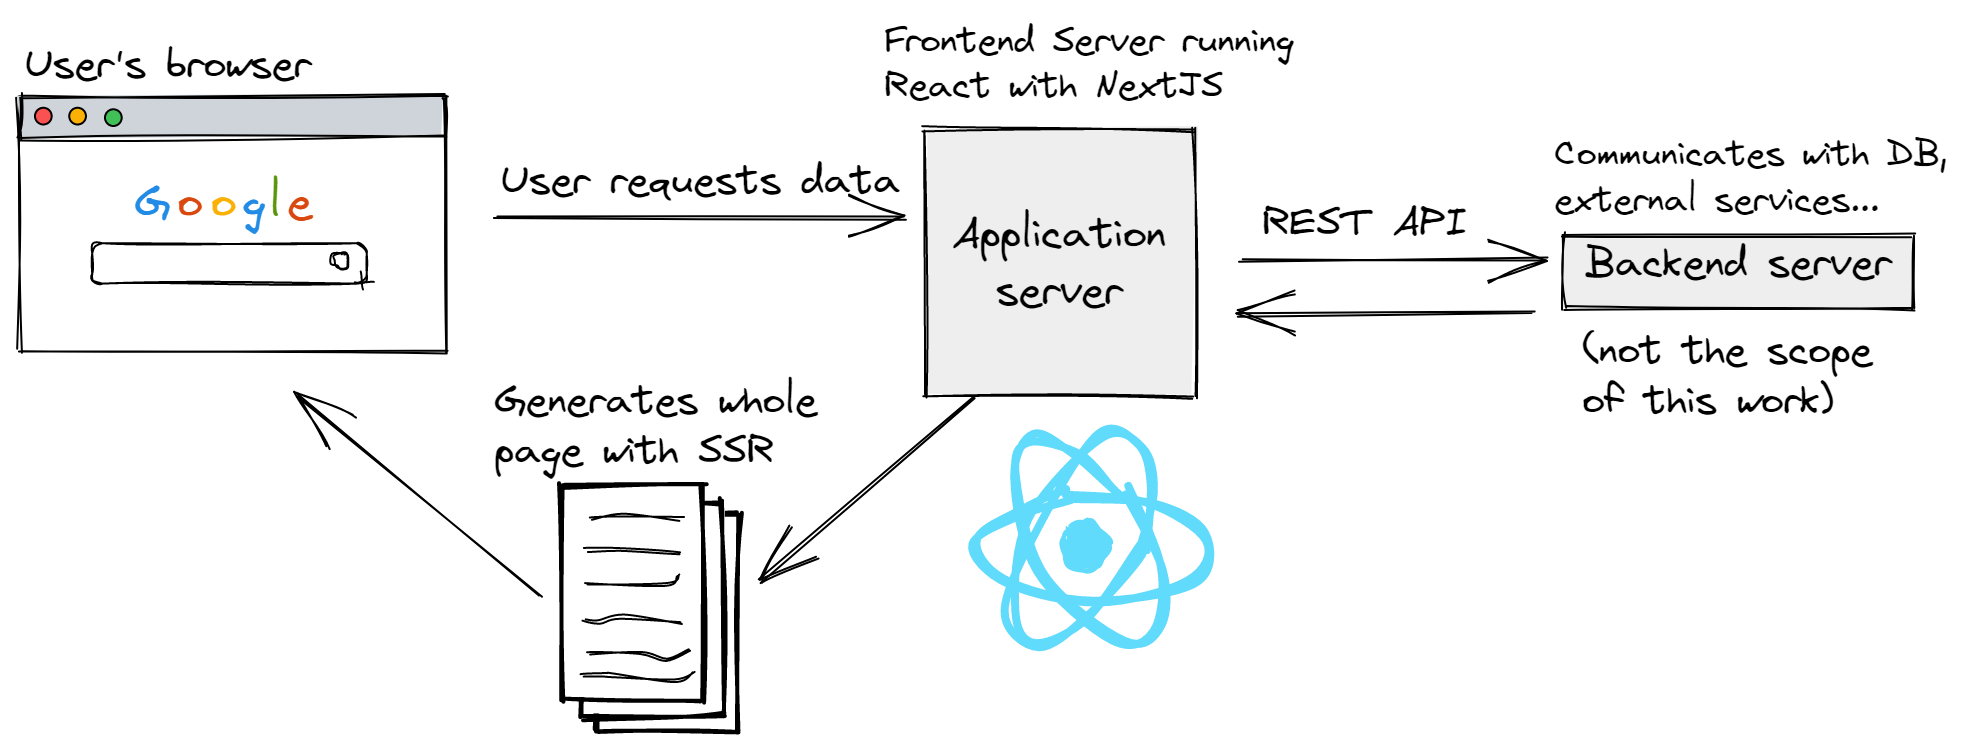
\includegraphics[width=14cm]{img/6-architecture.png}
      \end{center}
      \fonte{Author.}
    \end{figure}

    Regarding NextJS, it was chosen because it extends React by enabling \ac{SSR}\footnote{The term \ac{SSI} is used by \textcite{DBLP:journals/corr/abs-0801-2618}, but is interchangeable with \acl{SSR}.} capabilities. This greatly reduces loading times for the user, because the whole page document with its \ac{HTML} - the standard markup language for documents designed to be displayed in a web browser \cite{patel2013incremental} - tags are pre generated on the application server and delivered all at once when the page loads \cite{DBLP:journals/corr/abs-0801-2618}.

    However, this is not normally the case for React applications, which rely commonly on \ac{CSR}\footnote{The term \ac{CSI} is used by \textcite{DBLP:journals/corr/abs-0801-2618}, but is interchangeable with \acl{CSR}.}. With this approach, the React framework sends the bare minimum information needed in the first load, followed by a loading screen to the user until the page itself is generated locally in the user's browser \cite{DBLP:journals/corr/abs-0801-2618}. \Cref{fig:csr} and \Cref{fig:ssr} aim to illustrate this behavior.

    This approach has a number of drawbacks, including the inability to support users who do not have JavaScript enabled, potential security risks, much longer page load times, and negative effects on the site's overall \ac{SEO} \cite{Thakkar2020}.

    \begin{figure}[!htb]
      \caption{\acl{CSR}}\label{fig:csr}
      \begin{center}
        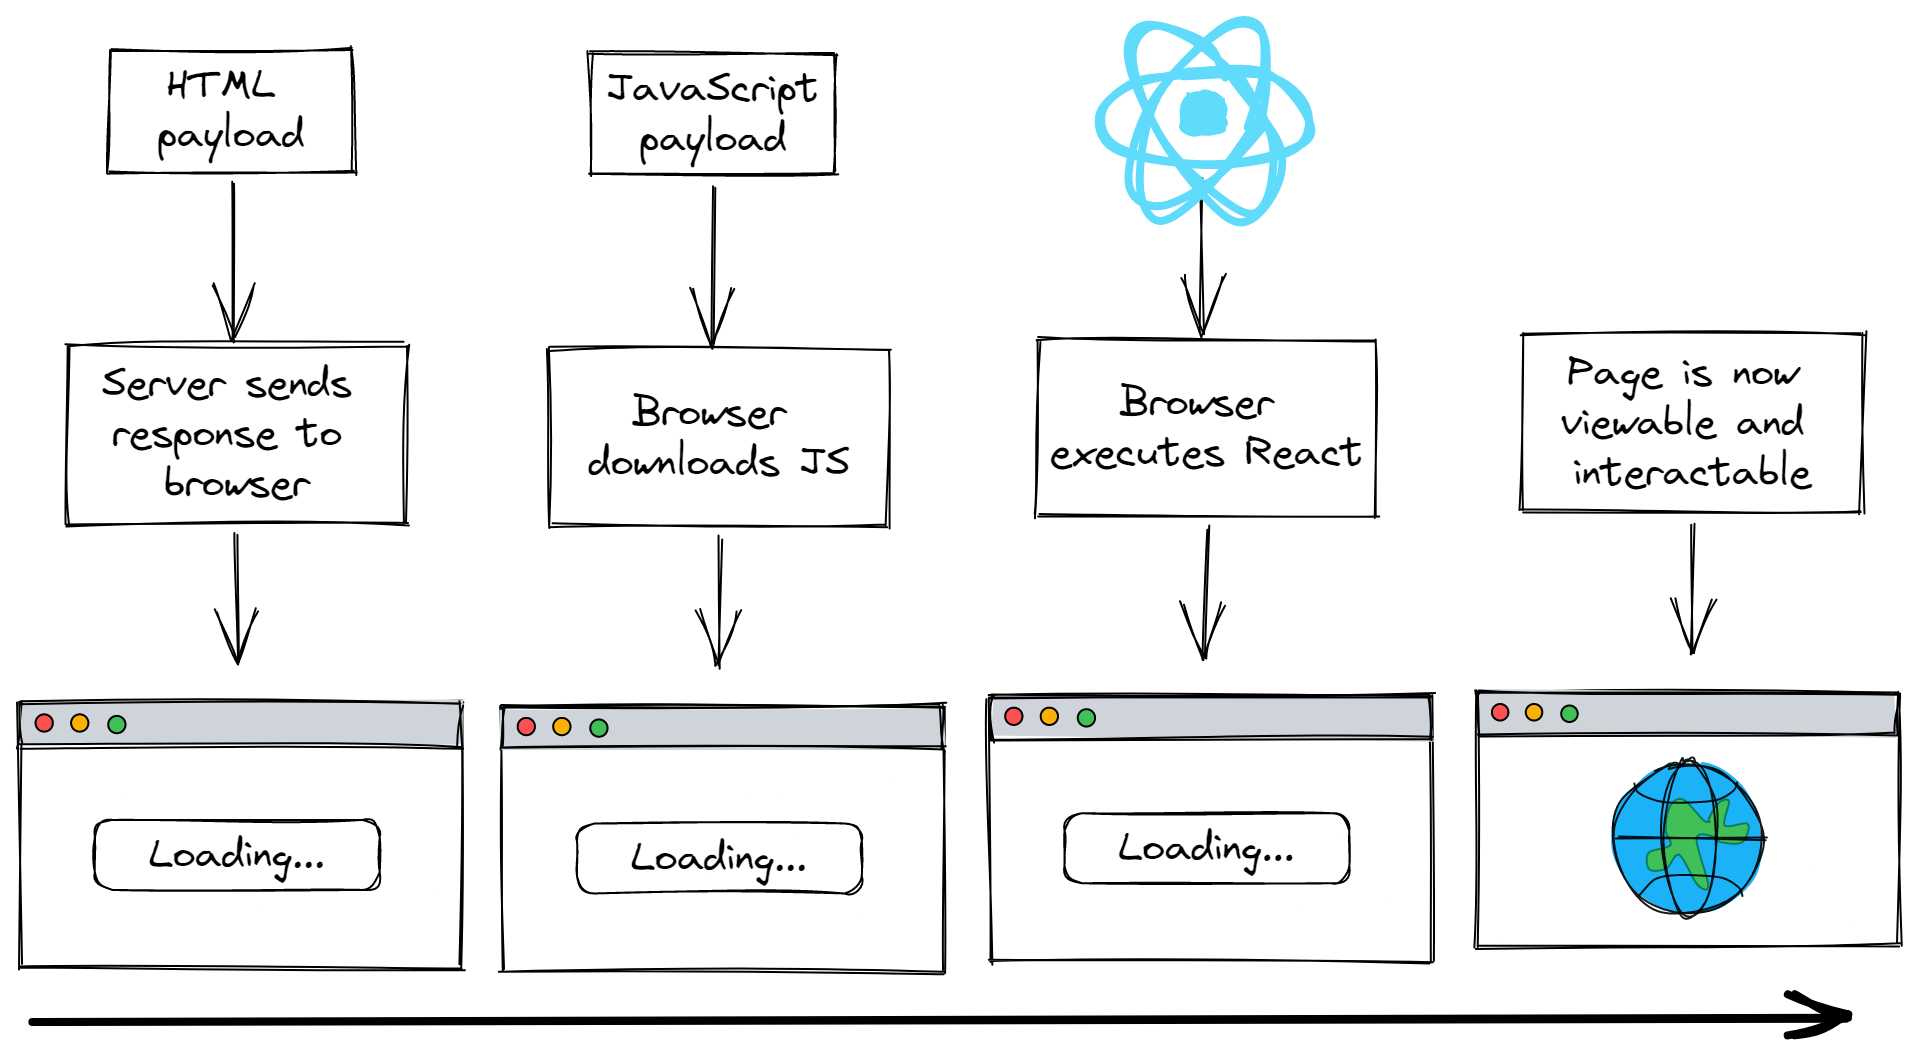
\includegraphics[width=14cm]{img/6-csr.png}
      \end{center}
      \fonte{Adapted from \cite{grigoryan_2017}.}
    \end{figure}

    \begin{figure}[!htb]
      \caption{\acl{SSR}}\label{fig:ssr}
      \begin{center}
        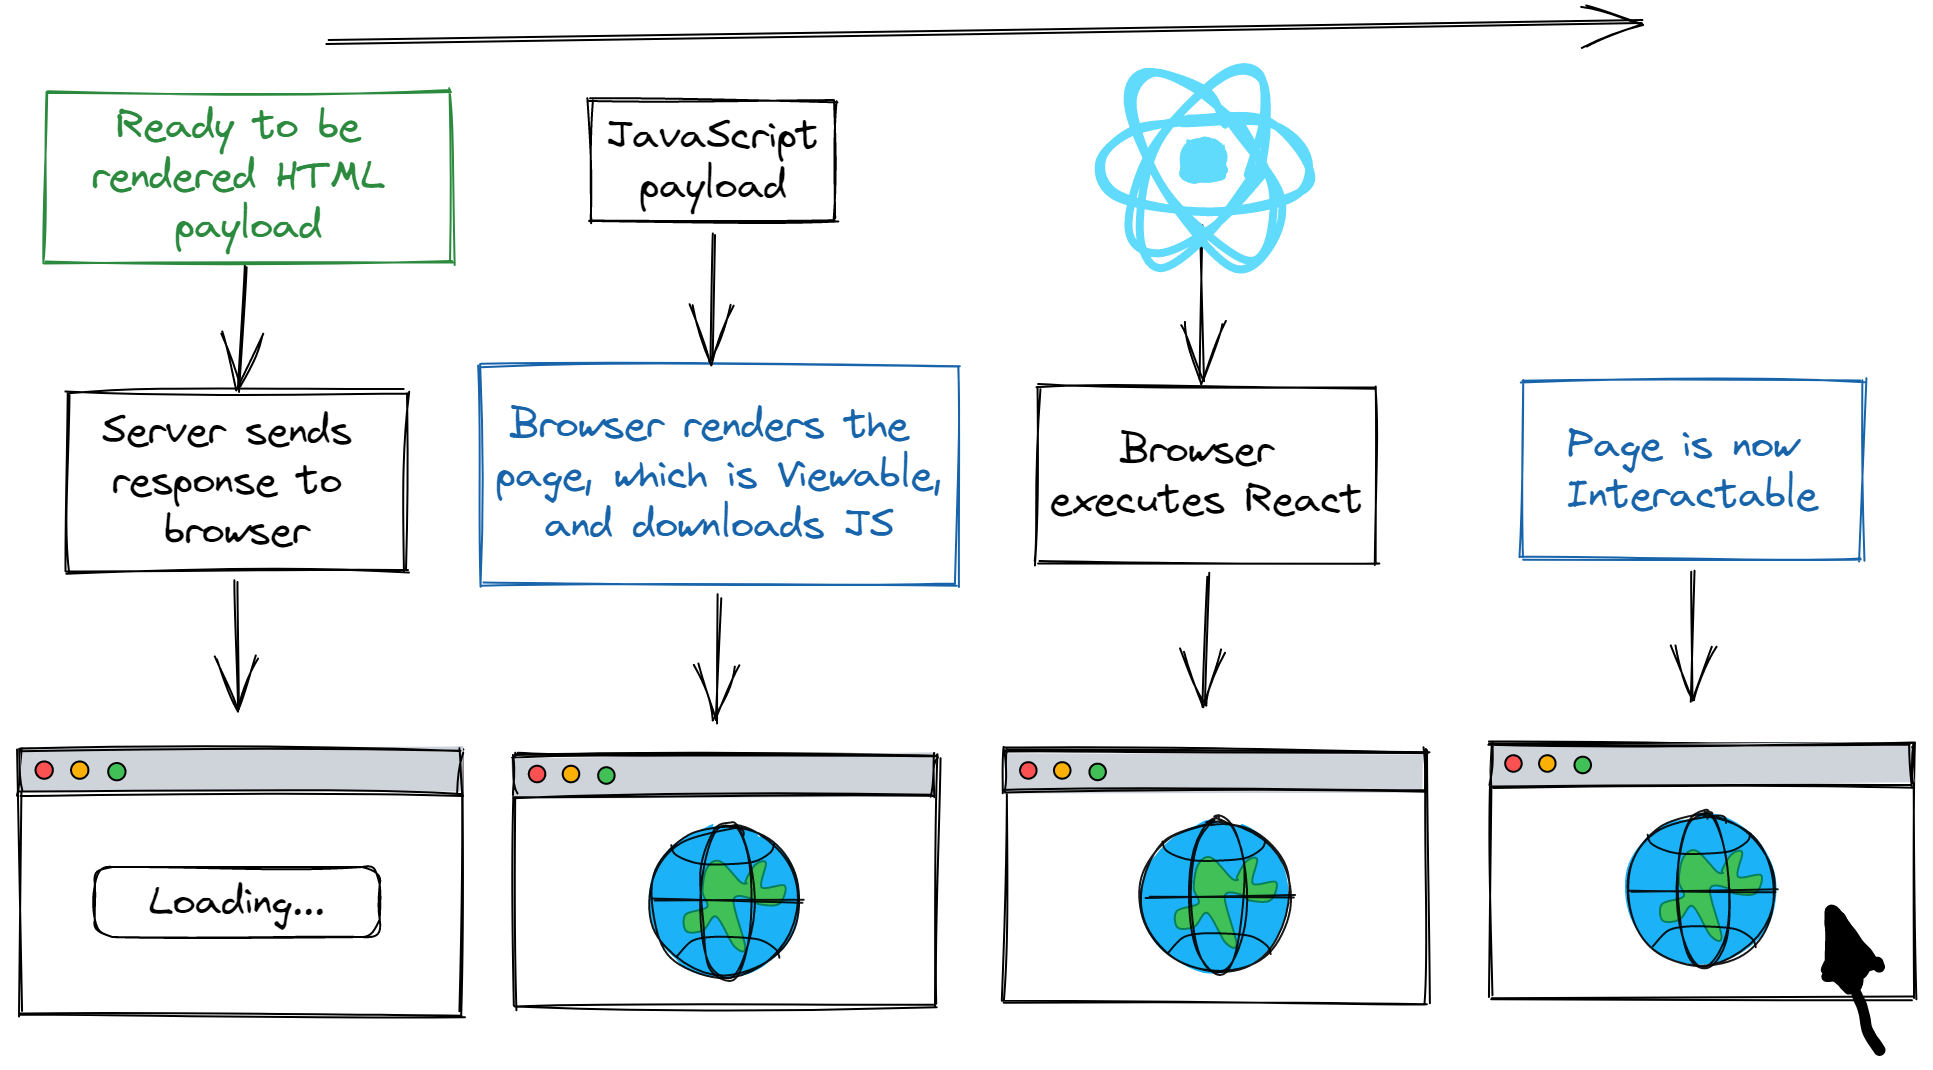
\includegraphics[width=14cm]{img/6-ssr.png}
      \end{center}
      \fonte{Adapted from \cite{grigoryan_2017}.}
    \end{figure}

  \item[\textbf{License:}] The front-end web application is licensed under the GNU General Public License v3.0, which is an open source license and is very permissive, allowing even for commercial use. It is very important to note, however, that any works or modifications must be licensed under the same license, while also making available their source code and that the distribution of closed source versions is prohibited. It also does not provide any kind of warranty or liability regarding the software \cite{gnugpl3}.
  \item[\textbf{Multiple Languages:}] The application will be translated to multiple languages, being available at first in Portuguese and English. While this does not hold much importance right now, as the current focus is to cater for the local Portuguese-speaking community, having this in mind since the beginning will save a lot of time in the future, if the software ever expands globally \cite{reynolds_2020}.
  \item[\textbf{Transparent Analytics:}] Analytics is used to identify, explain, and communicate significant trends in data. It also involves using data patterns to make smart decisions \cite{Kohavi02emergingtrends}. However, as opposed to collecting and tracking data using the commonest solution in the market, Google Analytics \cite{w3techs_2019}, it was decided that the web application should be privacy-friendly and user focused.

    Plausible was chosen, because they have proven that it is possible to measure a website's usage without utilizing cookies, collecting any \ac{PII} about the website's visitors, or collecting any personal data at all \cite{plausible_2022}. This is done through an analytics dashboard available publicly and accessible by anyone, which displays anonymous data about the traffic in the website. \Cref{fig:plausible} illustrates an example of this dashboard\footnote{The dashboard is available for anyone on their website, through \url{https://plausible.io/plausible.io}.}.

    \begin{figure}[!htb]
      \caption{Plausible Analytics Dashboard}\label{fig:plausible}
      \begin{center}
        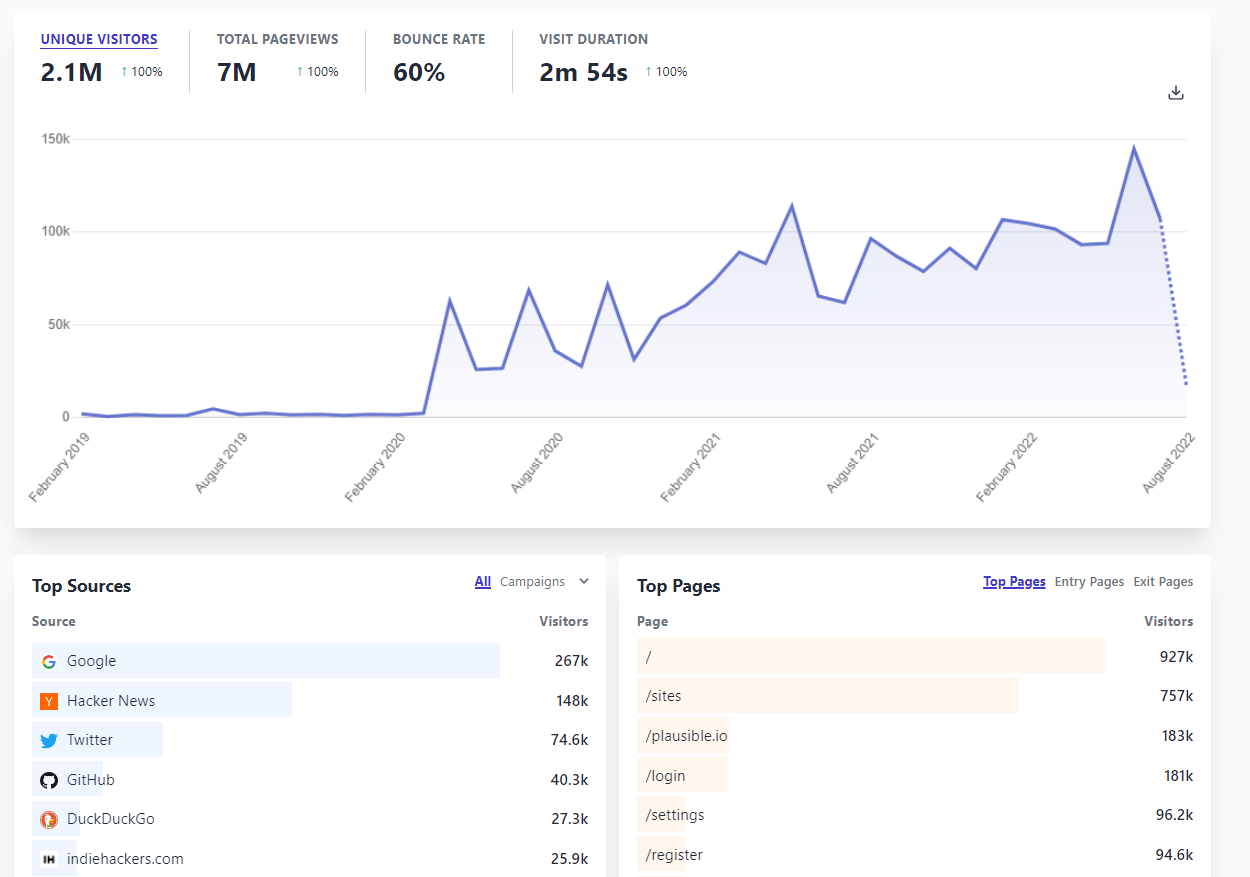
\includegraphics[width=16cm]{img/6-plausible.png}
      \end{center}
      \fonte{\cite{plausible_2022}}
    \end{figure}

\end{description}
